\documentclass[11pt]{article}
\usepackage[a4paper,margin=0.78in]{geometry}
\usepackage{amsmath,amssymb,amsthm,mathtools}
\usepackage{graphicx,enumitem,microtype}
\usepackage[dvipsnames]{xcolor}
\usepackage[colorlinks=true,linkcolor=MidnightBlue,citecolor=MidnightBlue,urlcolor=MidnightBlue]{hyperref}
\setlist{nosep,leftmargin=*}
\newtheorem{theorem}{Theorem}
\newtheorem{corollary}[theorem]{Corollary}
\newcommand{\T}{\mathbb T}
\newcommand{\C}{\mathbb C}
\newcommand{\Sph}{\mathbb S}
\newcommand{\F}{\mathcal F}
\newcommand{\one}{\mathbf 1}
\title{Periodic microlocal compactness forms retain the signed spectrum\\
\large Two counterexamples to the published Oscillation Lemma and an exact replacement}
\author{Autonomous solve-first investigation, lane 12}
\date{13 August 2026}

\begin{document}
\maketitle

\begin{abstract}
Rindler asks which formal microlocal compactness forms (MCFs) admit a
generating sequence.  We prove an exact formula for the basic realizable
class generated by bounded one-periodic profiles.  The formula is the signed
Fourier cross-spectrum of $h\circ w$ and $w$, not the Young-measure expression
stated in Lemma~4.1 of the source.  Two counterexamples are decisive.  A real
two-phase square wave makes the published formula twice the defining MCF
pairing.  A positive-frequency complex exponential has zero negative-cone
pairing although the published formula assigns it nonzero mass; hence no
scalar normalization repairs the claim.  The full generability problem is
not claimed, but any characterization must retain this signed cross-spectral
compatibility.
\end{abstract}

\section{Source question and source claim}

The source is F.~Rindler, \emph{Directional oscillations, concentrations,
and compensated compactness via microlocal compactness forms},
arXiv:1212.1430v3, published in \emph{Archive for Rational Mechanics and
Analysis} 215 (2015), 1--63 \cite{Rindler}.

After Example~5.8 (printed p.~38), the source observes that not every formal
MCF is generated and asks for a characterization of the generated subclass:

\begin{center}
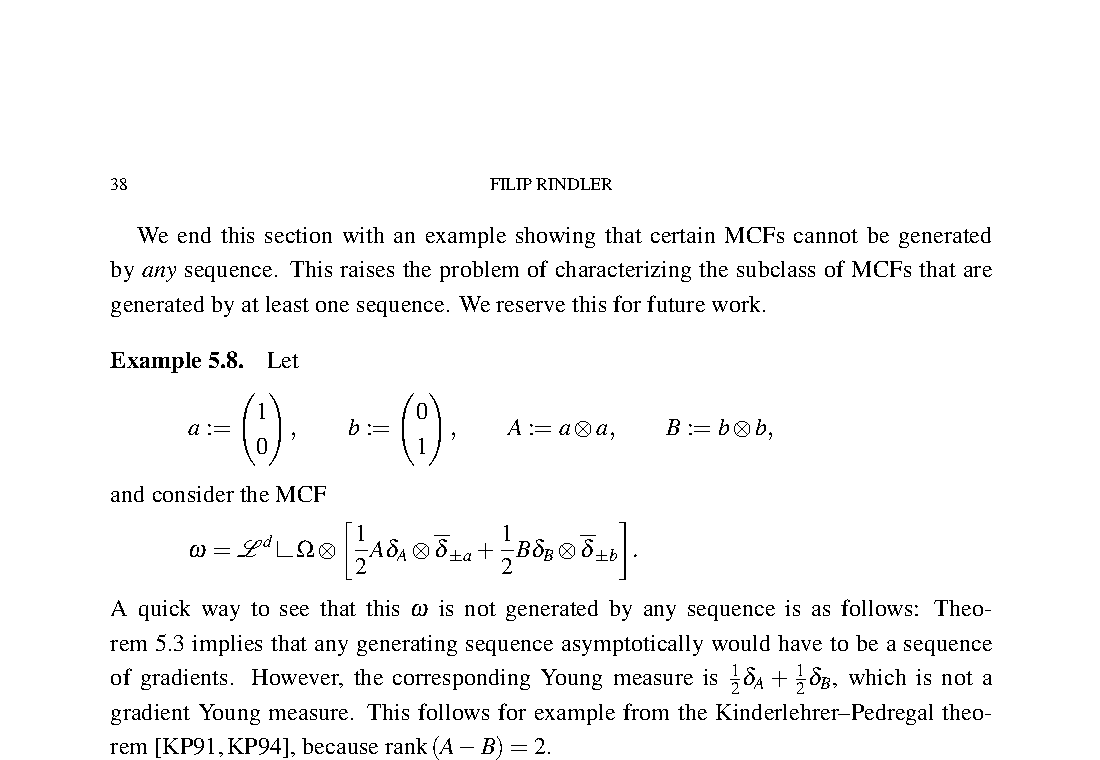
\includegraphics[width=0.94\textwidth]{figures/open_problem.png}
\end{center}

The basic asserted supply of generated forms is Lemma~4.1 (printed p.~28):

\begin{center}
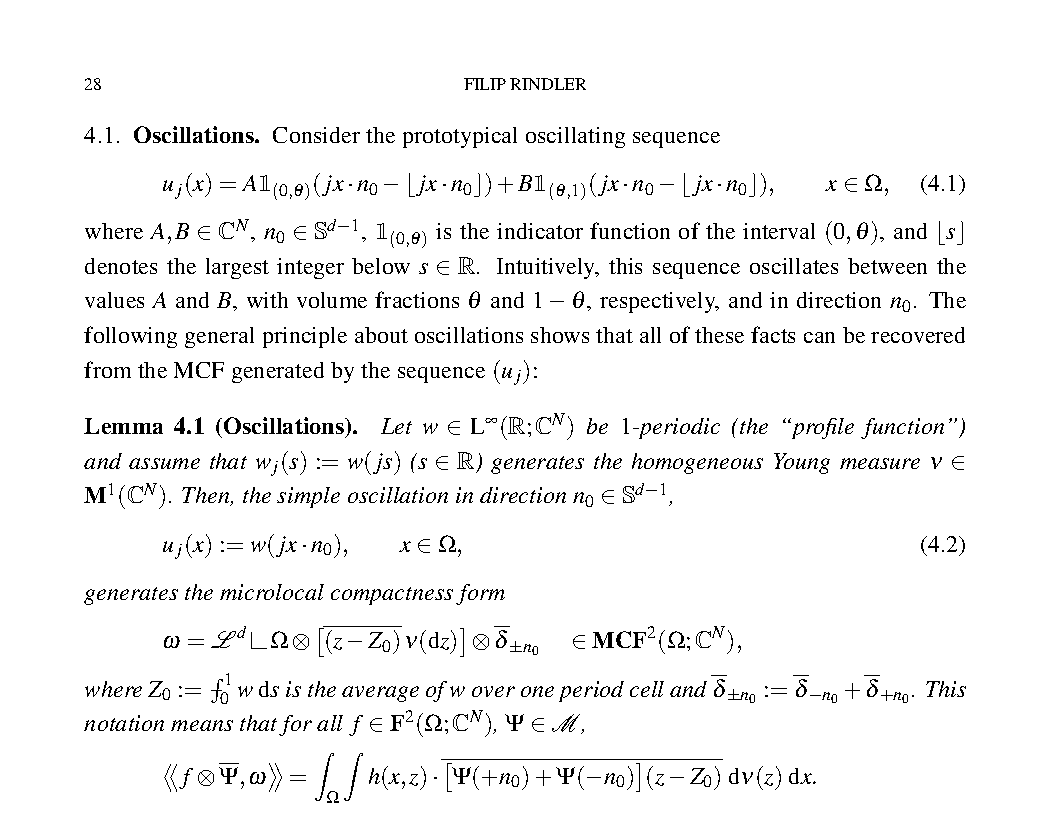
\includegraphics[width=0.94\textwidth]{figures/oscillation_lemma.png}
\end{center}

In the source notation, a bounded periodic profile $w$ with mean $Z_0$ and
Young measure $\nu$ is asserted to give, for
$u_j(x)=w(jx\cdot n_0)$,
\begin{equation}\label{eq:source}
 \langle\!\langle \phi h\otimes\overline\Psi,\omega\rangle\!\rangle
 =\int_\Omega\phi(x)\!\int h(z)\cdot
  \overline{[\Psi(n_0)+\Psi(-n_0)](z-Z_0)}\,d\nu(z)\,dx.
\end{equation}

\section{Idea of the proof}

The multiplier $\Psi$ sees the sign of every nonzero Fourier mode.  If
$c_k$ is the $k$th coefficient of $w$ and $a_k$ that of $h\circ w$, then
frequency separation pairs $a_k$ only with $c_k$, in direction
$\operatorname{sgn}(k)n_0$.  Formula \eqref{eq:source} instead replaces each
one-sided part by the complete defect $w-Z_0$; it therefore counts a real
two-phase defect twice and creates a nonexistent negative-frequency defect
for a positive-frequency complex wave.  Trigonometric polynomials give the
correct formula directly; $L^2$ approximation and Cauchy--Schwarz complete
the proof for bounded profiles.

\section{Exact periodic-profile formula}

Write $\T=\mathbb R/\mathbb Z$.  For $w\in L^\infty(\T;\C^N)$ and continuous
$h:\C^N\to\C^N$, define
\[
 c_k=\int_0^1w(s)e^{-2\pi i k s}\,ds,\qquad
 a_k=\int_0^1h(w(s))e^{-2\pi i k s}\,ds.
\]

\begin{theorem}[signed cross-spectrum formula]\label{thm:correct}
Let $\Omega\subset\mathbb R^d$ be bounded, $n_0\in\Sph^{d-1}$, and
$u_j(x)=w(jx\cdot n_0)$.  Let $\omega$ be the $2$-MCF generated by a
subsequence.  For every $\phi\in C_c^\infty(\Omega)$, every continuous $h$
(only its restriction to the bounded range of $w$ matters), and every
admissible matrix multiplier $\Psi$,
\begin{equation}\label{eq:correct}
 \langle\!\langle \phi h\otimes\overline\Psi,\omega\rangle\!\rangle
 =\left(\int_\Omega\phi(x)\,dx\right)
   \sum_{k\in\mathbb Z\setminus\{0\}}
   a_k\cdot\overline{\Psi(\operatorname{sgn}(k)n_0)c_k}.
\end{equation}
The series is absolutely convergent.  In particular the right side is
subsequence-independent.
\end{theorem}

\begin{proof}
First suppose that $w$ and $H:=h\circ w$ are trigonometric polynomials.
Localize inside $\Omega$ as in the source's multiplier-localization lemma,
and factor a dense collection of spatial tests as
$\phi=\phi_1\overline{\phi_2}$ with band-limited Schwartz factors.  Then
\[
 \F[\phi_1H(j\,\cdot\, n_0)](\xi)
 =\sum_k a_k\widehat\phi_1(\xi-jk n_0),\quad
 \F[\phi_2w(j\,\cdot\, n_0)](\xi)
 =\sum_l c_l\widehat\phi_2(\xi-jl n_0).
\]
For large $j$, distinct translated supports are disjoint, so only $k=l$
survives in the Parseval pairing.  The high-frequency cutoff removes
$k=l=0$.  On the translate indexed by $k\ne0$, the multiplier converges to
$\Psi(\operatorname{sgn}(k)n_0)$.  The remaining spatial integral is
$\int\phi$, proving \eqref{eq:correct} for trigonometric polynomials.

For general bounded $w$, both $w$ and $H$ lie in $L^2(\T)$.  Approximate each
by trigonometric polynomials.  Uniform $L^2$ multiplier bounds and periodic
averaging control the error in the defining pairing.  On the coefficient
side,
\[
 \sum_{k\ne0}|a_k|\,|\Psi(\operatorname{sgn}(k)n_0)c_k|
 \le \|\Psi\|_\infty\|(a_k)\|_{\ell^2}\|(c_k)\|_{\ell^2},
\]
so the series converges absolutely and the polynomial formulas pass to the
limit.  Density of the localized spatial tests gives all
$\phi\in C_c^\infty(\Omega)$.
\end{proof}

For $\Psi\equiv I$, Parseval reduces \eqref{eq:correct} to
\[
 \int_0^1h(w(s))\cdot\overline{w(s)-c_0}\,ds,
\]
the expected Young-measure defect.  It occurs once, not once in each cone.

\section{Two counterexamples}

\begin{corollary}[real two-phase contradiction]\label{cor:real}
Lemma~4.1 of \cite{Rindler} is false even for $d=N=1$, real-valued $w$, and
the constant multiplier.
\end{corollary}

\begin{proof}
Let $w=1$ on $(0,\tfrac12)$ and $w=-1$ on $(\tfrac12,1)$, periodically;
take $h(z)=z$ and $\Psi\equiv1$.  Its mean is zero and its Young measure is
$\nu=\tfrac12\delta_1+\tfrac12\delta_{-1}$.  By the MCF definition (or
\eqref{eq:correct}), the pairing is $\int_\Omega\phi$: the low-frequency
part is compact and $u_j\rightharpoonup0$, while $|u_j|=1$.  But
\eqref{eq:source} gives
\[
 \int_\Omega\phi\int z\,\overline{(1+1)z}\,d\nu(z)
 =2\int_\Omega\phi,
\]
a contradiction for any nonzero nonnegative $\phi\in C_c^\infty(\Omega)$.
\end{proof}

\begin{corollary}[one-sided contradiction]\label{cor:complex}
The failure is not repaired by inserting a factor $1/2$ in
$\overline\delta_{\pm n_0}$.
\end{corollary}

\begin{proof}
Take $d=N=1$, $w(s)=e^{2\pi i s}$, $h(z)=z$, and choose the multiplier on
$\Sph^0=\{-1,+1\}$ by $\Psi(+1)=0$, $\Psi(-1)=1$.  In
\eqref{eq:correct}, only $c_1=a_1=1$ is nonzero, so the pairing vanishes.
Equivalently, on $\Omega=(0,1)$ the zero extension satisfies
\[
 \widehat u_j(\xi)=\widehat{\one_{(0,1)}}(\xi-j),\qquad
 \int_{\xi<0}|\widehat u_j(\xi)|^2\,d\xi
 =\int_{\eta<-j}|\widehat{\one_{(0,1)}}(\eta)|^2\,d\eta\longrightarrow0.
\]
Thus its negative-frequency MCF component is zero.  Yet $Z_0=0$, the Young
measure is Haar probability on the unit circle, and \eqref{eq:source}
predicts $\int_\Omega\phi$.  The source formula loses the signed spectrum,
not merely a numerical factor.
\end{proof}

\section{Implications, verification, and scope}

The erroneous step is equation~(4.4) in the source proof: after localization
to one cone, it replaces the cone projection of $u_j-Z_0$ by the entire
$u_j-Z_0$.  The correct term is the corresponding one-sided Fourier part.
For a real two-state profile and affine tests, the familiar product formula
can be repaired by assigning half the variance to each sign.  For general
profiles there is no product of the Young measure with a fixed two-point
direction measure; the cross-spectrum \eqref{eq:correct} is essential.

The full characterization of all generated MCFs remains open.  The theorem
does provide an exact generated subclass and a necessary lesson for any
general answer: the recovered Young measure and an unsigned directional
support do not determine the nonlinear directional correlations.  Source
examples and lamination formulas that invoke Lemma~4.1 require re-audit; no
claim is made here about which later conclusions survive after correction.

The two counterexamples were checked both from the defining double limit and
from \eqref{eq:correct}; a finite Fourier verifier is included in the packet.
Exact-phrase, title, periodic-profile, correction, erratum, and generability
searches on 13 August 2026 found the source and author slides repeating the
same claim, but no published correction or full characterization.  Novelty
is plausible, not certified.  Human review should focus on the localization
step in Theorem~\ref{thm:correct} and on downstream uses of Lemma~4.1.

\begin{thebibliography}{9}
\bibitem{Rindler}
F. Rindler,
\emph{Directional oscillations, concentrations, and compensated compactness
via microlocal compactness forms},
Arch. Ration. Mech. Anal. 215 (2015), 1--63;
arXiv:1212.1430v3.
\end{thebibliography}

\end{document}
